\documentclass[a4paper]{article}
\usepackage[a4paper,margin=25mm]{geometry}
\usepackage{graphicx,subcaption}
\usepackage{amsmath,amsfonts}
\usepackage{qtree}
\usepackage{tikz}
\title{Notes on Sequence Modelling}
\author{G.A. Jarrad}
\usepackage{accents}
\newcommand{\rvec}[1]{\accentset{\leftarrow}{#1}}
\newcommand{\Bb}[1]{%
  \expandafter\def\csname#1#1\endcsname%
  {\ensuremath{\mathbb #1}}}
\Bb X\Bb S\Bb V\Bb Z
\newcommand{\up}{\!\uparrow}
\newcommand{\dn}{\downarrow\!}

\begin{document}
\maketitle
\numberwithin{equation}{section}
\numberwithin{figure}{section}
\numberwithin{table}{section}
\section{Random Sequence Processes}
\label{sec:random-processes}
Consider a random process $R$ that generates arbitrary-length sequences
of the form $\vec{R}=(R_1,R_2,\ldots,R_N)$, where $N=|\vec{R}|$ is a random variable governing
the length of a sequence, and $R_t$ is a random variable governing the value at {\em stage} $t$
of the sequence. This sequence process is graphically depicted in Figure~\ref{fig:R-process}.
\begin{figure}[hbt]
\centering
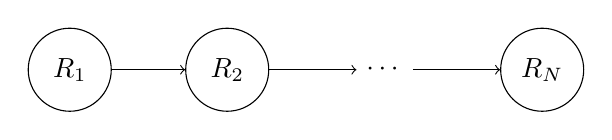
\begin{tikzpicture}[cnode/.style={draw,circle,minimum size=3em,inner sep=3pt}]
    \node[cnode] (1) at (0,0) {$R_1$};
    \node[cnode] (2) at (2, 0)  {$R_2$};
    \node (t) at (4, 0) {$\cdots$};
    \node[cnode] (n) at (6, 0)  {$R_N$};

    \draw[->] (1) edge (2) ;
    \draw[->] (2) edge (t) ;
    \draw[->] (t) edge (n) ;
\end{tikzpicture}
\caption{\em A random process $R$ for generating sequences of arbitrary length $N$. The arrows indicate transitions from one stage in the sequence to the next.}
\label{fig:R-process}
\end{figure}

We assume that each $R_t$ randomly takes some discrete or continuous value $r_t\in{\cal R}$,
and hence the probability (or probability density) of observing a particular
sequence $\vec{r}$ of length $n=|\vec{r}|$ is given by
\begin{eqnarray}
   p(\vec{R}\!=\!\vec{r}) & = & p(N=n)\,p(R_1\!=\!r_1,\ldots,R_n\!=\!r_n)\,.
\end{eqnarray}
In practice, this definition presupposes that we know we have observed a {\em complete} sequence that started
at stage 1 and ended at stage $n$.
Suppose instead that the sequence $\vec{r}$ was observed one stage at a time. How do we know if the
underlying process has actually terminated, or will instead
continue to generate another observed value $r_{n+1}$? 
Similarly, how do we know that the first observed value $r_1$ was not in fact
part of a longer, unobserved sequence of values?
We assume that the random process $R$ only ever produces complete sequences,
independently of the observation process, which might provide partial or complete sequences of values.
Furthermore, if the random process does not signal the start and end of generated sequences,
then an observed sequence might actually comprise a subsequence of multiple, contiguously generated sequences.

In order to handle such difficulties, we consider any arbitrary sequence $\vec{r}$ to be {\em incomplete},
and explicitly denote the corresponding, complete sequence by $\langle\vec{r}\rangle$.
We can now introduce the notion of {\em partially complete} sequences:
let  $\langle\vec{r}$ be a {\em start sequence} that has a definite start but an indefinite end;
and let $\vec{r}\rangle$ be an {\em end sequence} that has a definite end but an indefinite start.
Furthermore, if we know that all of the values of $\vec{r}$ are contiguous values of the same sequence,
then we can denote this by introducing additional, paired delimiters.
Thus, we use the symbol $\uparrow$ to indicate that the true sequence definitely does not end at the observed
value $r_n$, e.g.\ $\langle\vec{r}\up$, and the symbol $]$ to indicate that we are uncertain as to whether or not the
sequence ends at $r_n$, but definitely does not end at an earlier stage, e.g.\ $\langle\vec{r}]$.
Similarly, let $\downarrow$ indicate that the true sequence starts at an earlier stage than $r_1$, e.g.\ $\dn\vec{r}\rangle$,
and let $[$ indicate that the sequence might start at $r_1$ or at an earlier stage, e.g.\ $[\vec{r}\rangle$. Clearly, we may also
specify the remaining partial, contiguous sequences $[\vec{r}]$, $\dn\vec{r}]$, $[\vec{r}\up$ and $\dn\vec{r}\up$.

Under this augmented notation, knowledge about the start of a sequence can be encapsulated in 
a random indicator variable $\iota_{t-1}$, which takes on the value 1 if some observed $r_{t}$ is definitely the first stage in the
true sequence, or the value 0 if it is not. Similarly, the random indicator variable $\tau_{t+1}$
takes on the value 1 if $r_{t}$ is definitely the last stage in the true sequence, or the value 0 if it is not.
Notionally, the indicators $\iota_0$ and $\tau_{n+1}$ can be thought to correspond to pseudo-stages 0 and $n+1$, such that
the generated sequence is initiated at stage 0 and terminated at stage $N+1$.
This augmented random process is depicted in Figure~\ref{fig:random-process}. 
\begin{figure}[hbt]
\centering
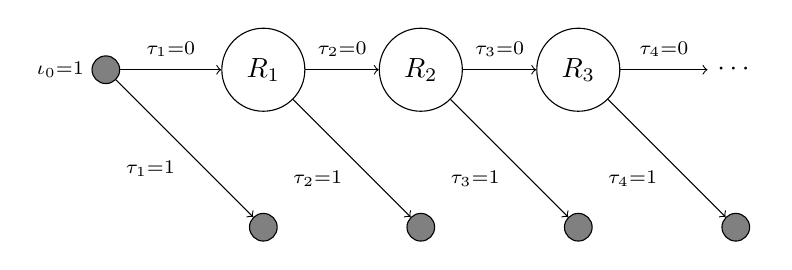
\begin{tikzpicture}[cnode/.style={draw,circle,minimum size=3em,inner sep=3pt}, onode/.style={fill=black!50, draw,circle,minimum size=1em}]
    \node (0i) at (-1,0) [right] {$\stackrel{\iota_0=1}{}$};
    \node[onode] (0) at (0,0) {};
    \node[cnode] (1) at (2,0) {$R_1$};
    \node[onode] (1t) at (2,-2) {};
    \node[cnode] (2) at (4, 0)  {$R_2$};
    \node[onode] (2t) at (4,-2) {};
    \node[cnode] (3) at (6, 0)  {$R_3$};
    \node[onode] (3t) at (6,-2) {};
    \node (t) at (8, 0) {$\cdots$};
    \node[onode] (tt) at (8, -2) {};

    \draw[->] (0) edge node [pos=0.5, above] {$\stackrel{\tau_1=0}{}$}  (1) ;
    \draw[->] (0) edge node [pos=0.5, below left] {$\stackrel{\tau_1=1}{}$} (1t) ;
    \draw[->] (1) edge node [pos=0.5, above] {$\stackrel{\tau_2=0}{}$}  (2) ;
    \draw[->] (1) edge node [pos=0.5, below left] {$\stackrel{\tau_2=1}{}$} (2t) ;
    \draw[->] (2) edge node [pos=0.5, above] {$\stackrel{\tau_3=0}{}$}  (3) ;
    \draw[->] (2) edge node [pos=0.5, below left] {$\stackrel{\tau_3=1}{}$} (3t) ;
    \draw[->] (3) edge node [pos=0.5, above] {$\stackrel{\tau_4=0}{}$}  (t) ;
    \draw[->] (3) edge node [pos=0.5, below left] {$\stackrel{\tau_4=1}{}$} (tt) ;
\end{tikzpicture}
\caption{\em A random process for generating complete sequences of arbitrary length,
with explicit stages for sequence initiation and termination. Multiple arrows exiting from a node indicate
different possible (mutually exclusive) stage transition pathways.}
\label{fig:random-process}
\end{figure}

The probability of a given complete sequence $\langle\vec{r}\rangle$ is now defined as
\begin{eqnarray}
   p(\langle\vec{r}\rangle)
& = & p(\iota_0\!=\!1,\tau_1\!=\!0,R_1=r_1,\ldots,\tau_n\!=\!0,R_n=r_n,\tau_{n+1}\!=\!1)
\,,
\end{eqnarray}
such that 
\begin{eqnarray}
   p(N\!=\!n) & = &  p(\iota_0\!=\!1,\tau_1\!=\!0,\ldots,\tau_n\!=\!0,\tau_{n+1}\!=\!1)\,.
\end{eqnarray}
This has the form of a generalised Bernoulli sequence.
Conversely, the probability of the start sequence $\langle\vec{r}\up$ is
\begin{eqnarray}
p(\langle\vec{r}\up) 
& = & p(\iota_0\!=\!1,\tau_1\!=\!0,R_1\!=\!r_1,\ldots,\tau_n\!=\!0,R_n\!=\!r_n,\tau_{n+1}\!=\!0)\,,
\end{eqnarray}
and the probability of the end sequence $\dn\vec{r}\rangle$ is
\begin{eqnarray}
p(\dn\vec{r}\rangle)
& = & p(\iota_0\!=\!0,\tau_1\!=\!0,R_1\!=\!r_1,\ldots,\tau_n\!=\!0,R_n\!=\!r_n,\tau_{n+1}\!=\!1)\,.
\end{eqnarray}
We may also write the probability of the ambiguous start sequence $\langle\vec{r}]$ as
\begin{eqnarray}
p(\langle\vec{r}]) 
& = & p(\iota_0\!=\!1,\tau_1\!=\!0,R_1\!=\!r_1,\ldots,\tau_n\!=\!0,R_n\!=\!r_n,\tau_{n+1}\!=\!*)\,,
\end{eqnarray}
where $\tau_{n+1}=*$ is just a shorthand to indicate that we are uncertain of the true value of $\tau_{n+1}$;
probabilistically, the term has no effect and may be dropped.
Likewise, the probability of the end sequence $[\vec{r}\rangle$ is
\begin{eqnarray}
p([\vec{r}\rangle)
& = & p(\iota_0\!=\!*,\tau_1\!=\!0,R_1\!=\!r_1,\ldots,\tau_n\!=\!0,R_n\!=\!r_n,\tau_{n+1}\!=\!1)\,.
\end{eqnarray}
The likelihood of the other types of partial sequences can similarly be defined.
Generically, we can write the likelihood of any complete or partially complete sequence as
\begin{eqnarray}
p(\underline{\iota},\vec{r},\underline{\tau})
& = & p(\iota_0\!=\!\underline{\iota},\tau_1\!=\!0,R_1\!=\!r_1,\ldots,\tau_n\!=\!0,R_n\!=\!r_n,\tau_{n+1}\!=\!\underline{\tau})\,,
\end{eqnarray}
where the observed sequence-start indicator $\underline{\iota}\in\{0,1,*\}$ corresponds to the delimiters
$\downarrow$ ,$\langle$, and $[$, respectively, and the observed sequence-end indicator
$\bar{\tau}\in\{0,1,*\}$ corresponds to the delimiters $\uparrow$, $\rangle$, and $]$, respectively.

%%%%%%%%%%%%%%%%%%%%%%%%%%%%%%%%%%%
\section{Markov Sequence Processes}
\label{sec:markov-processes}
In Section~\ref{sec:random-processes} we defined a random process $R$ and the sequences it generates.
We now assume that the process is also {\em causal}, meaning that each stage of a sequence,
including the termination stage, depends only on the preceding stages.
This causal process, depicted in Figure~\ref{fig:causal-process}, is simply the random process from
Figure~\ref{fig:random-process} with additional, explicit dependencies (in the form of dashed arrows).
\begin{figure}[hbt]
\centering
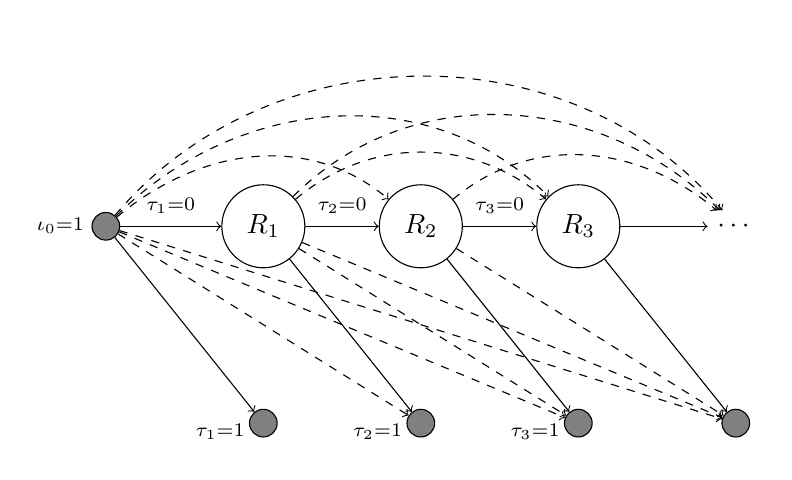
\begin{tikzpicture}[cnode/.style={draw,circle,minimum size=3em,inner sep=3pt}, onode/.style={fill=black!50, draw,circle,minimum size=1em}]
    \node (0i) at (-1,0) [right] {$\stackrel{\iota_0=1}{}$};
    \node[onode] (0) at (0,0) {};
    \node[cnode] (1) at (2,0) {$R_1$};
    \node[onode] (1t) at (2,-2.5) {};
    \node[cnode] (2) at (4, 0)  {$R_2$};
    \node[onode] (2t) at (4,-2.5) {};
    \node[cnode] (3) at (6, 0)  {$R_3$};
    \node[onode] (3t) at (6,-2.5) {};
    \node (t) at (8, 0) {$\cdots$};
    \node[onode] (tt) at (8, -2.5) {};

    \draw[->] (0) edge node [pos=0.5, above] {$\stackrel{\tau_1=0}{}$}  (1) ;
    \draw[->] (0) edge node [pos=1, below left] {$\stackrel{\tau_1=1}{}$} (1t) ;
    \draw[->] (1) edge node [pos=0.5, above] {$\stackrel{\tau_2=0}{}$}  (2) ;
    \draw[->] (1) edge node [pos=1, below left] {$\stackrel{\tau_2=1}{}$} (2t) ;
    \draw[->] (2) edge node [pos=0.5, above] {$\stackrel{\tau_3=0}{}$}  (3) ;
    \draw[->] (2) edge node [pos=1, below left] {$\stackrel{\tau_3=1}{}$} (3t) ;
    \draw[->] (3) edge node [pos=0.5, above] {}  (t) ;
    \draw[->] (3) edge node [pos=0.5, below left] {} (tt) ;

   \begin{scope}[dashed]
    \draw[->] (0) to (2t) ;
    \draw[->] (0) to[out=40,in=140] (2) ;
    \draw[->] (0) to[out=45,in=135] (3) ;
    \draw[->] (0) to[out=50,in=130] (t) ;
    \draw[->] (0) to (3t) ;
    \draw[->] (0) to (tt) ;
    \draw[->] (1) to (tt) ;
    \draw[->] (1) to (3t) ;
    \draw[->] (2) to (tt) ;
    \draw[->] (1) to[out=40,in=140] (3) ;
    \draw[->] (1) to[out=45,in=135] (t) ;
    \draw[->] (2) to[out=40,in=140] (t) ;
   \end{scope}
\end{tikzpicture}
\caption{\em A fully-dependent, causal process for generating complete sequences of arbitrary length.
Solid arrows indicate possible stage transitions. 
Both dashed arrows and solid arrows indicate parent--child dependencies, such that the child node is conditionally dependent on the parent and all other ancestral nodes.}
\label{fig:causal-process}
\end{figure}

Hence, under the Markov assumption of conditional independence,
the causal sequence process leads to the full-dependency conditional model
\begin{eqnarray}
p(\underline{\iota},\vec{r},\underline{\tau}) & = &
p(\iota_0\!=\!\underline{\iota})
\,p(\tau_1\!=\!0\,|\,\iota_0\!=\!\underline{\iota})
\,p(R_1\!=\!r_1\,|\,\iota_0\!=\!\underline{\iota},\tau_1\!=\!0)
\,p(\tau_2\!=\!0\,|\,\iota_0\!=\!\underline{\iota},\tau_1\!=\!0,R_1\!=\!r_1)
\nonumber\\&&
{}\times p(R_2\!=\!r_2\,|\,\iota_0\!=\!\underline{\iota},\tau_1\!=\!0,R_1\!=\!r_1,\tau_2\!=\!0)
\cdots
p(R_n\!=\!r_n\,|\,\iota_0\!=\!1,\ldots,\tau_{n}\!=\!0)
\nonumber\\&&
{}\times p(\tau_{n+1}\!=\!1\:|\;\iota_0\!=\!1,\ldots,R_n\!=\!r_n)
\,.
\label{eq:temporal-model-full}
\end{eqnarray}
We can generalise this model by first defining a forward observation sub-sequence $\vec{r}_t=(r_1,r_2,\ldots,r_t)$,
for $t=1,2,\ldots,n$, where $\vec{r}_0$ is taken to be the empty sub-sequence by definition.
 For later convenience, we also define the backward observation sub-sequence $\rvec{r}_t=(r_t,r_{t+1},\ldots,r_n)$,
for $t=n,n-1,\ldots,1$; likewise, $\rvec{r}_{n+1}$ is an empty sub-sequence.
Hence, we obtain
\begin{eqnarray}
p(\underline{\iota},\vec{r},\underline{\tau}) & = &
p(\iota_0\!=\!\underline{\iota})
%\,p(\tau_1\!=\!0\,|\,\iota_0\!=\!\underline{\iota})\,p(R_1\!=\!r_1\,|\,\iota_0\!=\!\underline{\iota},\tau_1\!=\!0)
\prod_{t=1}^{n}\left\{p(\tau_t\!=\!0\,|\,\iota_0\!=\!\underline{\iota},\vec{\tau}_{t-1}\!=\!\vec{0}_{t-1},
\vec{R}_{t-1}\!=\!\vec{r}_{t-1})\right.
\nonumber\\&&
\hspace*{20mm}{}\times \left.
p(R_t\!=\!r_t\,|\,\iota_0\!=\!\underline{\iota},\vec{\tau}_t\!=\!\vec{0}_t,\vec{R}_{t-1}\!=\!\vec{r}_{t-1})\right\}
\nonumber\\&&
{}\times p(\tau_{n+1}\!=\!\bar{\tau}\:|\;\iota_0\!=\!\underline{\iota},\vec{\tau}_n\!=\!\vec{0},\vec{R}_n\!=\!\vec{r}_n)
\,.
\label{eq:temporal-model}
\end{eqnarray}

In practice, the full-dependency model is usually considerably simplified by 
dropping some of the explicit (dashed) dependencies.
For example, one might limit the 
conditionality on past values to a maximum of $m$ depenencies.
This leads to the so-called {\em $m$-th order Markov model}.
An example from the realm of natural language understanding is the lexicographical analysis of the character
sequences of words using bigrams (pairs of adjacent characters, corresponding to $m=1$), and trigrams 
(triples of adjacent characters, corresponding to $m=2$), et cetera.
The second-order Markov sequence process is depicted in Figure~\ref{fig:causal-process-2}.
\begin{figure}[hbt]
\centering
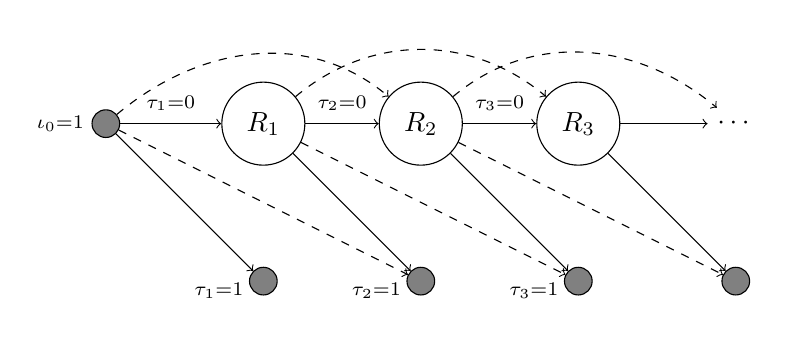
\begin{tikzpicture}[cnode/.style={draw,circle,minimum size=3em,inner sep=3pt}, onode/.style={fill=black!50, draw,circle,minimum size=1em}]
    \node (0i) at (-1,0) [right] {$\stackrel{\iota_0=1}{}$};
    \node[onode] (0) at (0,0) {};
    \node[cnode] (1) at (2,0) {$R_1$};
    \node[onode] (1t) at (2,-2) {};
    \node[cnode] (2) at (4, 0)  {$R_2$};
    \node[onode] (2t) at (4,-2) {};
    \node[cnode] (3) at (6, 0)  {$R_3$};
    \node[onode] (3t) at (6,-2) {};
    \node (t) at (8, 0) {$\cdots$};
    \node[onode] (tt) at (8, -2) {};

    \draw[->] (0) edge node [pos=0.5, above] {$\stackrel{\tau_1=0}{}$}  (1) ;
    \draw[->] (0) edge node [pos=1, below left] {$\stackrel{\tau_1=1}{}$} (1t) ;
    \draw[->] (1) edge node [pos=0.5, above] {$\stackrel{\tau_2=0}{}$}  (2) ;
    \draw[->] (1) edge node [pos=1, below left] {$\stackrel{\tau_2=1}{}$} (2t) ;
    \draw[->] (2) edge node [pos=0.5, above] {$\stackrel{\tau_3=0}{}$}  (3) ;
    \draw[->] (2) edge node [pos=1, below left] {$\stackrel{\tau_3=1}{}$} (3t) ;
    \draw[->] (3) edge node [pos=0.5, above] {}  (t) ;
    \draw[->] (3) edge node [pos=0.5, below left] {} (tt) ;

   \begin{scope}[dashed]
    \draw[->] (0) to (2t) ;
    \draw[->] (0) to[out=40,in=140] (2) ;
    \draw[->] (1) to (3t) ;
    \draw[->] (2) to (tt) ;
    \draw[->] (1) to[out=40,in=140] (3) ;
    \draw[->] (2) to[out=40,in=140] (t) ;
   \end{scope}
\end{tikzpicture}
\caption{\em A second-order Markov process for generating complete sequences of arbitrary length.}
\label{fig:causal-process-2}
\end{figure}

In the special case of $m=1$, the first-order Markov model takes on the restricted conditional form
\begin{eqnarray}
p(\underline{\iota},\vec{r},\underline{\tau}) & = &
p(\iota_0\!=\!\underline{\iota})\,p(\tau_1\!=\!0\,|\,\iota_0\!=\!\underline{\iota})
p(R_1\!=\!r_1\,|\,\iota_0\!=\!\underline{\iota},\tau_1\!=\!0)
\nonumber\\&&
{}\times\prod_{t=2}^{n}\left\{p(\tau_t\!=\!0\,|\,R_{t-1}\!=\!r_{t-1})
\,p(R_t\!=\!r_t\,|\,\tau_t\!=\!0,R_{t-1}\!=\!r_{t-1})\right\}
\nonumber\\&&
{}\times p(\tau_{n+1}\!=\!\underline{\tau}\:|\;R_n\!=\!r_n)
\,.
\end{eqnarray}
This is just a Markov interpretation of the random process depicted in Figure~\ref{fig:random-process},
where each stage directly depends only on the previous stage {\em and} on the transition path between the two adjacent stages.

\section{Stateful Markov Sequence Processes}
Consider the first-order Markov process $R$ depicted in Figure~\ref{fig:random-process}.
Suppose now that the random variable $R_t$ at stage $t$ can be decomposed into the tuple
$R_t=(S_t,X_t)$, where $S_t$ is a random variable taking values $s_t\in{\cal S}$, and $X_t$
is a random variable taking values $x_t\in{\cal X}$.
We may call $S_t$ the {\em state} of the process at stage $t$, and $X_t$ its {\em value}.
As is usual, we presuppose that the stage transitions in the sequence generating process are primarily between states, e.g.\ from $S_{t-1}$ to $S_t$.
It follows that the value is generated after the state has been determined, i.e.\ $X_t$ depends upon $S_t$.
Keeping to the first-order Markov interpretation of stage-to-stage dependencies leads to
the {\em stateful} process depicted in Figure~\ref{fig:stateful-process}, with full cross-dependencies between $(S_t,X_t)$ and
$(S_{t+1},X_{t+1})$.
\begin{figure}[hbt]
\centering
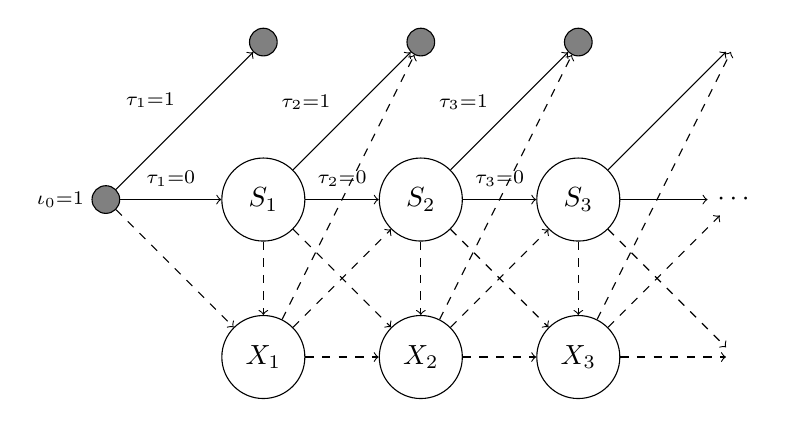
\begin{tikzpicture}[cnode/.style={draw,circle,minimum size=3em,inner sep=3pt}, onode/.style={fill=black!50, draw,circle,minimum size=1em}]
    \node (0i) at (-1,0) [right] {$\stackrel{\iota_0=1}{}$};
    \node[onode] (0) at (0,0) {};
    \node[cnode] (1) at (2,0) {$S_1$};
    \node[cnode] (1x) at (2,-2) {$X_1$};
    \node[onode] (1t) at (2,2) {};
    \node[cnode] (2) at (4, 0)  {$S_2$};
    \node[cnode] (2x) at (4, -2)  {$X_2$};
    \node[onode] (2t) at (4,2) {};
    \node[cnode] (3) at (6, 0)  {$S_3$};
    \node[cnode] (3x) at (6, -2)  {$X_3$};
    \node[onode] (3t) at (6,2) {};
    \node (t) at (8, 0) {$\cdots$};
    \node (tx) at (8, -2)  {};
    \node (tt) at (8,2) {};

    \draw[->] (0) edge node [pos=0.5, above] {$\stackrel{\tau_1=0}{}$}  (1) ;
    \draw[->] (0) edge node [pos=0.5, above left] {$\stackrel{\tau_1=1}{}$} (1t) ;
    \draw[->] (1) edge node [pos=0.5, above] {$\stackrel{\tau_2=0}{}$}  (2) ;
    \draw[->] (1) edge node [pos=0.4, above left] {$\stackrel{\tau_2=1}{}$} (2t) ;
    \draw[->] (2) edge node [pos=0.5, above] {$\stackrel{\tau_3=0}{}$}  (3) ;
    \draw[->] (2) edge node [pos=0.4, above left] {$\stackrel{\tau_3=1}{}$} (3t) ;
    \draw[->] (3) edge (t) ;
    \draw[->] (3) edge (tt) ;

   \begin{scope}[dashed]
    \draw[->] (0) to (1x) ;
    \draw[->] (1) to (1x) ;
    \draw[->] (1) to (2x) ;
    \draw[->] (1x) to (2) ;
    \draw[->] (1x) to (2x) ;
    \draw[->] (1x) to (2t) ;
    \draw[->] (2) to (2x) ;
    \draw[->] (2) to (3x) ;
    \draw[->] (2x) to (3) ;
    \draw[->] (2x) to (3x) ;
    \draw[->] (2x) to (3t) ;
    \draw[->] (3) to (3x) ;
    \draw[->] (3) to (tx) ;
    \draw[->] (3x) to (tx) ;
    \draw[->] (3x) to (t) ;
    \draw[->] (3x) to (tt) ;
   \end{scope}
\end{tikzpicture}
\caption{\em A random process for generating complete, stateful  sequences of arbitrary length,
with explicit cross-dependencies between adjacent stages.}
\label{fig:stateful-process}
\end{figure}

Hence, the fully-structured stateful model is now given by
\begin{eqnarray}
p(\underline{\iota},\vec{s},\vec{x},\underline{\tau}) & = & 
p(\iota_0\!=\!\underline{\iota})\,p(\tau_1\!=\!0\,|\,\iota_0\!=\!\underline{\iota})
\,p(S_1\!=\!s_1\,|\,\iota_0\!=\!\underline{\iota},\tau_1\!=\!0)
\nonumber\\&&{}\times
\,p(X_1\!=\!x_1\,|\,S_1\!=\!s_1,\iota\!=\!\underline{\iota},\tau_1\!=\!0)
\nonumber\\&&
{}\times\prod_{t=2}^{n}\left\{p(\tau_t\!=\!0\,|\,S_{t-1}\!=\!s_{t-1},X_{t-1}\!=\!x_{t-1})\right.
\nonumber\\&&\hspace*{10mm}{}\times\left.
\,p(S_t\!=\!s_t\,|\,\tau_t\!=\!0,,S_{t-1}\!=\!s_{t-1},X_{t-1}\!=\!x_{t-1})\right.
\nonumber\\&&\hspace*{10mm}{}\times\left.
\,p(X_t\!=\!x_t\,|\,S_t\!=\!s_t,S_{t-1}\!=\!s_{t-1},X_{t-1}\!=\!x_{t-1})\right\}
\nonumber\\&&
{}\times p(\tau_{n+1}\!=\!\bar{\tau}\,|\,S_n\!=\!s_n,X_n\!=\!x_n)
\,.
\end{eqnarray}
Conditioning the state $S_t$ on both the previous state $S_{t-1}$ and its value $X_{t-1}$
can be useful in some circumstances, e.g.\ in sequence classification problems.
However, due to the increased complexity of such models, it is more usual to further restrict the stateful process
by also imposing the first-order Markov assumption at the level
of the state--value dependencies themselves. In terms of the process depicted in Figure~\ref{fig:stateful-process},
this means retaining only direct node-to-node dependencies, rather than stage-to-stage dependencies.
This restricted process is depicted in Figure~\ref{fig:stateful-1-process}.
\begin{figure}[hbt]
\centering
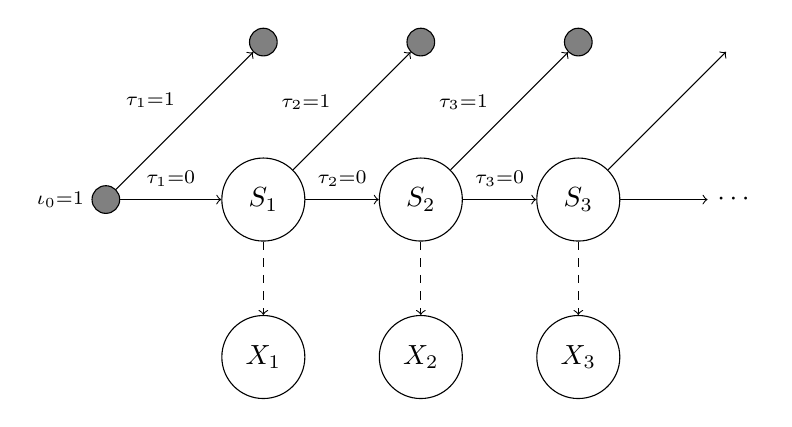
\begin{tikzpicture}[cnode/.style={draw,circle,minimum size=3em,inner sep=3pt}, onode/.style={fill=black!50, draw,circle,minimum size=1em}]
    \node (0i) at (-1,0) [right] {$\stackrel{\iota_0=1}{}$};
    \node[onode] (0) at (0,0) {};
    \node[cnode] (1) at (2,0) {$S_1$};
    \node[cnode] (1x) at (2,-2) {$X_1$};
    \node[onode] (1t) at (2,2) {};
    \node[cnode] (2) at (4, 0)  {$S_2$};
    \node[cnode] (2x) at (4, -2)  {$X_2$};
    \node[onode] (2t) at (4,2) {};
    \node[cnode] (3) at (6, 0)  {$S_3$};
    \node[cnode] (3x) at (6, -2)  {$X_3$};
    \node[onode] (3t) at (6,2) {};
    \node (t) at (8, 0) {$\cdots$};
    \node (tx) at (8, -2)  {};
    \node (tt) at (8,2) {};

    \draw[->] (0) edge node [pos=0.5, above] {$\stackrel{\tau_1=0}{}$}  (1) ;
    \draw[->] (0) edge node [pos=0.5, above left] {$\stackrel{\tau_1=1}{}$} (1t) ;
    \draw[->] (1) edge node [pos=0.5, above] {$\stackrel{\tau_2=0}{}$}  (2) ;
    \draw[->] (1) edge node [pos=0.4, above left] {$\stackrel{\tau_2=1}{}$} (2t) ;
    \draw[->] (2) edge node [pos=0.5, above] {$\stackrel{\tau_3=0}{}$}  (3) ;
    \draw[->] (2) edge node [pos=0.4, above left] {$\stackrel{\tau_3=1}{}$} (3t) ;
    \draw[->] (3) edge (t) ;
    \draw[->] (3) edge (tt) ;

   \begin{scope}[dashed]
    \draw[->] (1) to (1x) ;
    \draw[->] (2) to (2x) ;
    \draw[->] (3) to (3x) ;
   \end{scope}
\end{tikzpicture}
\caption{\em A first-order Markov process for generating complete, stateful  sequences of arbitrary length.}
\label{fig:stateful-1-process}
\end{figure}

The corresponding sequence model is now given by
\begin{eqnarray}
p(\underline{\iota},\vec{s},\vec{x},\underline{\tau}) & = & 
p(\iota_0\!=\!\underline{\iota})\,p(\tau_1\!=\!0\,|\,\iota_0\!=\!\underline{\iota})
\,p(S_1\!=\!s_1\,|\,\iota_0\!=\!\underline{\iota},\tau_1\!=\!0)
\,p(X_1\!=\!x_1\,|\,S_1\!=\!s_1)
\nonumber\\&&
{}\times\prod_{t=2}^{n}\left\{p(\tau_t\!=\!0\,|\,S_{t-1}\!=\!s_{t-1})
\,p(S_t\!=\!s_t\,|\,\tau_t\!=\!0,,S_{t-1}\!=\!s_{t-1})\right.
\nonumber\\&&\hspace*{10mm}{}\times\left.
\,p(X_t\!=\!x_t\,|\,S_t\!=\!s_t)\right\}
\;p(\tau_{n+1}\!=\!\bar{\tau}\,|\,S_n\!=\!s_n)
\,.
\label{eq:stateful-1-model}
\end{eqnarray}
%Observe that the $\tau_1$ dependency can additionally be dropped in practice,
%since zero-length sequences convey little information, and are in fact undetectable if the
%generating process does not explicitly indicate the start and end of sequences.
So far, we have made no assumption as to whether the states take continuous values or discrete values.
In the next section, we consider the important sub-class of models where the states are discrete-valued.

\section{Discrete-state Sequence Models}\label{sec:discrete-state}

Consider the stateful, first-order Markov process depicted by Figure~\ref{fig:stateful-1-process}.
Let us now restrict our attention to the class of corresponding sequence models where
the state $S_t$ at any stage $t$ may now only take {\em discrete} values in the set 
${\cal S}=\{\sigma_1,\sigma_2,\ldots,\sigma_S\}$.
Hence, the sequence of states may arbitrarily be specified as $\vec{s}=(\sigma_{i_1},\sigma_{i_2},\ldots,\sigma_{i_n})$,
where each $i_t\in\{1,2,\ldots,S\}$.
In the event that a particular state $S_t$ is unobserved, we say that the state is {\em missing} or {\em hidden},
and denote $i_t=*$ and $s_t=*$. In the situation where all values of $\vec{s}$ are unobserved,
the sequence model~\eqref{eq:stateful-1-model} is known as a {\em hidden-state Markov model} (HMM).

The sequence model~\eqref{eq:stateful-1-model}
may now be explicitly conditioned on a general parameter $\theta$
that governs the various discrete state distributions. Each term in the model depends directly on the stage index $t$ and 
indirectly on the state index $i_t$. 
Furthermore, each term represents either the initial state, the terminal state, or the non-terminal transitions
between states at adjacent stages. Hence, let $\theta=(\Pi,\Gamma,\Omega)$, 
such that the probability of an arbitrary, observed\footnote{We assume that all observed sequences are non-zero in length,
since zero-length sequences are typically unobservable unless the generating process explicitly signals the start
and end of each sequence. The modelling of zero-length sequences will require an extra parameter.} sequence (with no hidden states) is given by
\begin{eqnarray}
p(\underline{\iota},\vec{s},\vec{x},\underline{\tau}\,|\,\theta) & = & \pi_{\underline{\iota},1,i_1}\,o_{1,i_1}(x_1)\left\{\prod_{t=1}^{n-1}\omega_{0,t,i_t}\,\Gamma_{t,i_t,i_{t+1}}\,o_{t+1,i_{t+1}}(x_{t+1})
\right\}\,\omega_{\underline{\tau},n,i_n}
\,.
\label{eq:p_s_x_g_theta}
\end{eqnarray}
The initial state $S_1$ of the sequence at stage $t=1$ is governed by the parameter $\vec{\pi}$, where
\begin{eqnarray}
  \pi_{0,t,i} & = & p(\iota_{t-1}\!=\!0\,|\,\theta)\,p(\tau_t\!=\!0\,|\,\iota_{t-1}\!=\!0,\theta)
      \,p(S_t\!=\!\sigma_{i}\,|\,\iota_{t-1}\!=\!0,\tau_t\!=\!0,\theta)\,,
\\
  \pi_{1,t,i} & = & p(\iota_{t-1}\!=\!1\,|\,\theta)\,p(\tau_t\!=\!0\,|\,\iota_{t-1}\!=\!1,\theta)
      \,p(S_t\!=\!\sigma_{i}\,|\,\iota_{t-1}\!=\!1,\tau_t\!=\!0,\theta)\,,
\end{eqnarray}
and
\begin{eqnarray}
  \pi_{*,t,i} & = & p(\iota_{t-1}\!=\!*\,|\,\theta)\,p(\tau_t\!=\!0\,|\,\iota_{t-1}\!=\!*,\theta)
      \,p(S_t\!=\!\sigma_{i}\,|\,\iota_{t-1}\!=\!*,\tau_t\!=\!0,\theta)
\nonumber\\& = &
  p(\tau_t\!=\!0,S_t\!=\!\sigma_i\,|\,\theta)~=~\pi_{0,t,i}+\pi_{1,t,i}\,.
\end{eqnarray}
Observe that each state $S_t$ for $t>1$ is a non-initial state, governed by $\pi_{0,t,i_t}$. However, such terms do
not explicitly appear in model~\eqref{eq:p_s_x_g_theta}, except if $\underline{\iota}\ne 1$, 
since they are already accounted for by the state transitions.
These implicit terms become important when it comes to parameter estimation (see Section~\ref{sec:estimate-known}).

The terminal state $S_n$ at stage $t=n$ is likewise governed by the parameter $\vec{\omega}$, where
\begin{eqnarray}
  \omega_{0,t,i} & = & p(\tau_{t+1}\!=\!0\,|\,S_t\!=\!\sigma_{i},\theta)\,,
\\
  \omega_{1,t,i} & = & p(\tau_{t+1}\!=\!1\,|\,S_t\!=\!\sigma_{i},\theta)\,,
\end{eqnarray}
and
\begin{eqnarray}
  \omega_{*,t,i} & = & p(\tau_{t+1}\!=\!*\,|\,S_t\!=\!\sigma_{i},\theta)
~=~\omega_{0,t,i}+\omega_{1,t,i}~=~1\,.
\end{eqnarray}
Observe that each state $S_t$ for $t<n$ is a non-terminal state, and is explicitly modelled by the term
$\omega_{0,t,i_t}$.

Lastly, the permissible transitions between the states $S_t$ and $S_{t+1}$ of consecutive stages $t$ and $t+1$ are governed by
the parameter $\Gamma$, where
\begin{eqnarray}
  \Gamma_{t,i,j} & = & p(S_{t+1}\!=\!\sigma_{j}\,|\,S_t\!=\!\sigma_{i},\tau_{t+1}\!=\!0,\theta)\,.
\end{eqnarray}
Note that the model also includes the likelihood of each observed value $x_t$ at stage $t$, for $t=1,2,\ldots,n$.
This so-called {\em data likelihood} is governed by the separate model
\begin{eqnarray}
  o_{t,i}(x) & = & p(X_t\!=\!x\,|\,S_t\!=\!\sigma_{i},\theta) \hspace*{5mm}\forall x\in{\cal X}\,.
\end{eqnarray}
We do not, however, explicitly declare the parameterisation structure of this likelihood model (see Section~\ref{sec:discrete-x} for a plausible model if $X_t$ takes discrete values). 
It suffices for our calculations that each $o_{t,i_t}(x_t)$ is available when required.

Finally, note that in the situtation where any state in the observed state sequence $\vec{s}$ is hidden, we have to marginalise model~\eqref{eq:p_s_x_g_theta} over each such missing state. Hence, in general, we may define
\begin{eqnarray}
   p(\underline{\iota},\vec{s},\vec{x},\underline{\tau}\,|\,\theta) 
& = & 
   \sum_{i_1'=1}^{S}\delta(i_1'\!=\!i_1)\sum_{i_2'=1}^{S}\delta(i_2'\!=\!i_2)\cdots\sum_{i_n'=1}^{S}\delta(i_n'\!=\!i_n)\,
\nonumber\\&&\hspace*{10mm}\pi_{\underline{\iota},1,i_1'}\,o_{1,i_1'}(x_1)\,
\left\{\prod_{t=1}^{n-1}\omega_{0,t,i_t'}\,\Gamma_{t,i_t',i_{t+1}'}\,o_{t+1,i_{t+1}'}(x_{t+1})
\right\}\,\omega_{\underline{\tau},n,i_n'}
\,,
\label{eq:p_s_x_g_theta:gen}
\end{eqnarray}
where $\delta(\cdot)$ is an indicator function taking the value $1$ (or $0$) if its argument is true (or false).
Note that if $S_t$ is a hidden state, then $i_t=*$ and $\delta(i_t'\!=\!*)=1$ for all $i_t'\in\{1,2,\ldots,S\}$; otherwise, the summation over $i_t'$ collapses to the observed value $i_t$.
The observation likelihood given by model~\eqref{eq:p_s_x_g_theta:gen} can be efficiently computed by an
extension of the forward--backward algorithm, described in the next section.

\subsection{Modified Forward--Backward Algorithm}\label{sec:forward-backward}

The sequence model~\eqref{eq:p_s_x_g_theta:gen} can be efficiently evaluated by marginalising over the state of each stage
in turn, using a modification of the {\em forward--backward algorithm} to include knowledge of
sequence initiation and termination.
 The forward pass involves first summing over all terms containing $i_1'$, then over all remaining terms containing $i_2'$,
and so on up to summing over $i_n'$. This is equivalent to evaluating the reordered model
\begin{eqnarray}
   p(\underline{\iota},\vec{s},\vec{x},\underline{\tau}\,|\,\theta) 
& = & 
   \left\{\sum_{i_n'=1}^{S}\delta(i_n'\!=\!i_n)
%\left\{\sum_{i_{n-1}'=1}^{S}\delta(i_{n-1}'\!=\!i_{n-1})\right.
\cdots
\right\{\sum_{i_2'=1}^{S}\delta(i_2'\!=\!i_2)
\nonumber\\&&
\hspace*{10mm}{}\times
\left\{\sum_{i_1'=1}^{S}\delta(i_1'\!=\!i_1)\,
\pi_{\underline{\iota},1,i_1'}\,o_{1,i_1'}(x_1)\,\omega_{0,1,i_1'}\,\Gamma_{1,i_1',i_{2}'}\right\}
\nonumber\\&&
\left.\rule{0pt}{7mm}
o_{2,i_{2}'}(x_{2})\omega_{0,2,i_{2}'}\,\Gamma_{2,i_{2}',i_{3}'}\right\}
\cdots
%\left.\rule{0pt}{7mm}\omega_{0,n-1,i_{n-1}'}\,\Gamma_{n-1,i_{n-1}',i_{n}'}\right\}
\left.\rule{0pt}{7mm}\,o_{n,i_{n}'}(x_{n})
\,\omega_{\underline{\tau},n,i_n'}\right\}
\,.
\label{eq:forward}
\end{eqnarray}
Conversely, the backaward pass reverses the order of evaluation, first summing over all terms containing $i_n'$,
and then over all remaining terms containing $i_{n-1}'$, and so on down to summing over $i_1'$.
This is equivalent to evaluating the reordered model
\begin{eqnarray}
   p(\underline{\iota},\vec{s},\vec{x},\underline{\tau}\,|\,\theta) 
& = & 
   \left\{\sum_{i_1'=1}^{S}\delta(i_1'\!=\!i_1)\,
\pi_{\underline{\iota},1,i_1'}\,o_{1,i_1'}(x_1)\,\omega_{0,1,i'_{1}}\,
\cdots\right.
\nonumber\\&&
{}\times\left\{\sum_{i_{n-1}'=1}^{S}\delta(i_{n-1}'\!=\!i_{n-1})\,
\Gamma_{n-2,i_{n-2}',i_{n-1}'}\,o_{n-1,i_{n-1}'}(x_{n-1})\,\omega_{0,n-1,i'_{n-1}}\right.
\nonumber\\&&
\hspace*{4mm}{}\times
\left.\rule{0pt}{7mm}\left\{\sum_{i_n'=1}^{S}\delta(i_n'\!=\!i_n)\,
\Gamma_{n-1,i_{n-1}',i_{n}'}\,o_{n,i_{n}'}(x_{n})
\,\omega_{\underline{\tau},n,i_n'}\right\}\right\}
\cdots\left.\rule{0pt}{7mm}\right\}
\,.
\label{eq:backward}
\end{eqnarray}

A more efficient mechanism for evaluation comes from making use of the first-order Markov dependencies.
Notionally, from the process depicted in Figure~\ref{fig:stateful-1-process}, we may arbitrarily consider the transition from 
some stage $t$ to stage $t+1$,
and partition the sequence into: (i) past values from the initial node up to and including $S_t$ and $X_t$;
and (ii) future values from $S_{t+1}$ and $X_{t+1}$ up to and including the terminal node.
Note that the termination or non-termination of stage $t$ is governed by $\tau_{t+1}$, which is
therefore a future value.
The Markov dependency then implies that the future values are conditioned only on state $S_t$
via $\tau_{t+1}$ and $S_{t+1}$.
Hence, remembering that notionally $s_t=\sigma_{i_t}$, model~\eqref{eq:p_s_x_g_theta:gen} reduces to
\begin{eqnarray}
   p(\underline{\iota},\vec{s},\vec{x},\underline{\tau}\,|\,\theta) 
& = &
   \sum_{i=1}^{S}p(S_t\!=\!\sigma_{i},\underline{\iota},\vec{s},\vec{x},\underline{\tau}\,|\,\theta) 
\nonumber\\& = & 
   \sum_{i=1}^{S}\delta(i\!=\!i_t)\,p(\underline{\iota},\vec{s}_{t-1}\circ\sigma_{i}\circ\rvec{s}_{t+1},\vec{x},\underline{\tau}\,|\,\theta) 
\nonumber\\& = & 
   \sum_{i=1}^{S}\delta(i\!=\!i_t)\,p(\underline{\iota},\vec{s}_{t-1}\circ\sigma_{i},\vec{x}_t\,|\,\theta) 
\,p(\dn\rvec{s}_{t+1},\rvec{x}_{t+1},\underline{\tau}\,|\,S_t=\sigma_{i},\theta) 
\nonumber\\& = &
  \sum_{i=1}^{S}\delta(i\!=\!i_t)\,\alpha_{t,i}\,\beta_{t,i}\,,
\label{eq:forward-backward}
\end{eqnarray}
where $\circ$ represents sequence concatenation.
The forward step $\alpha_{t,i}$ is defined as
\begin{eqnarray}
   \alpha_{t,i} & = & p(\underline{\iota},\vec{s}_{t-1}\circ\sigma_{i},\vec{x}_t\,|\,\theta) 
\nonumber\\& = &
   p(\underline{\iota},\vec{s}_{t-1}\circ\sigma_{i},\vec{x}_{t-1}\,|\,\theta) \,p(X_t\!=\!x_t\,|\,S_t\!=\!\sigma_{i'_t},\theta)
\nonumber\\& = &
   \bar{\alpha}_{t,i}\,o_{t,i}(x_t)\,,
\label{eq:alpha}
\end{eqnarray}
where $\bar{\alpha}_{t,i}$ is recursively defined as
\begin{eqnarray}
   \bar{\alpha}_{t,i} & = & p(\underline{\iota},\vec{s}_{t-1}\circ\sigma_{i},\vec{x}_{t-1}\,|\,\theta) 
\nonumber\\& = &
   \sum_{j=1}^{S}p(S_{t-1}\!=\!\sigma_j,\underline{\iota},\vec{s}_{t-1}\circ\sigma_{i},\vec{x}_{t-1}\,|\,\theta) 
\nonumber\\& = &
   \sum_{j=1}^{S}\delta(j=i_{t-1})\,p(\underline{\iota},\vec{s}_{t-2}\circ\sigma_{j}\circ\sigma_{i},\vec{x}_{t-1}\,|\,\theta) 
\nonumber\\& = &
   \sum_{j=1}^{S}\delta(j=i_{t-1})\,p(\underline{\iota},\vec{s}_{t-2}\circ\sigma_{j},\vec{x}_{t-1}\,|\,\theta) 
      \,p(\tau_t\!=\!0\,|\,S_{t-1}\!=\!\sigma_j,\theta)
\nonumber\\&&
    \hspace*{5mm}{}\times\,p(S_t\!=\!\sigma_i\,|\,\tau_{t}\!=\!0,S_{t-1}\!=\!\sigma_j,\theta)
\nonumber\\& = &
   \sum_{j=1}^{S}\delta(j=i_{t-1})\,\alpha_{t-1,j}\,\omega_{0,t-1,j}\,\Gamma_{t-1,j,i}\,,
\label{eq:alpha-bar}
\end{eqnarray}
for $t=2,3,\ldots,n$. The forward pass commences with the first step
\begin{eqnarray}
  \alpha_{1,i} & = & p(\underline{\iota},S_1=\sigma_{i},X_1\!=\!x_1\,|\,\theta) 
\nonumber\\& = & 
  p(\iota_0\!=\!\underline{\iota})\,p(\tau_1\!=\!0\,|\,\iota\!=\!\underline{\iota},\theta)
\,p(S_1\!=\!\sigma_i\,|\,\iota_0\!=\!\underline{\iota},\tau_1\!=\!0,\theta)\,p(X_1\!=\!x_1\,|\,S_1\!=\!\sigma_i,\theta)
\nonumber\\& = & 
  \pi_{\underline{\iota},1,i}\,o_{1,i}(x_1)
\,.
\label{eq:alpha_1}
\end{eqnarray}
Hence, observe that $\alpha_{2,i'_2}$, is just
the entire summation over $i'_1$ from the forward model~\eqref{eq:forward}.
Also note that the standard forward pass derivation commences with the equivalent of $\pi_{*,1,i}$ and does not include the
$\delta(\cdot)$ or $\omega$ terms.

Conversely to the forward pass, the backward step $\beta_{t,i}$ is defined as
\begin{eqnarray}
   \beta_{t,i} & = & p(\dn\rvec{s}_{t+1},\rvec{x}_{t+1},\underline{\tau}\,|\,S_t\!=\!\sigma_{i},\theta) 
\nonumber\\& = &
  p(\tau_{t+1}\!=\!0\,|\,S_t\!=\!\sigma_i,\theta)\,p(\rvec{s}_{t+1},\rvec{x}_{t+1},\underline{\tau}\,|\,\tau_{t+1}\!=\!0,S_t\!=\!\sigma_{i},\theta) 
\nonumber\\& = &
  \omega_{0,t,i}\,\bar{\beta}_{t,i}\,,
\label{eq:beta}
\end{eqnarray}
where
\begin{eqnarray}
   \bar{\beta}_{t,i} & = & p(\rvec{s}_{t+1},\rvec{x}_{t+1},\underline{\tau}\,|\,\tau_{t+1}\!=\!0,S_t\!=\!\sigma_{i},\theta) 
\nonumber\\& = &
  \sum_{j=1}^{S} p(S_{t+1}\!=\!\sigma_j,\rvec{s}_{t+1},\rvec{x}_{t+1},\underline{\tau}\,|\,\tau_{t+1}\!=\!0,S_t\!=\!\sigma_{i},\theta) 
\nonumber\\& = &
  \sum_{j=1}^{S}\delta(j\!=\!i_{t+1})\, p(\sigma_j\circ\rvec{s}_{t+2},x_{t+1}\circ\rvec{x}_{t+2},\underline{\tau}\,|\,\tau_{t+1}\!=\!0,S_t\!=\!\sigma_{i},\theta) 
%\nonumber\\& = &
 % \sum_{j=1}^{S}\delta(j\!=\!i_{t+1})\, p(S_{t+1}\!=\!\sigma_j,X_{t+1}\!=\!x_{t+1}\,|\,\tau_{t+1}\!=\!0,S_t\!=\!\sigma_{i},\theta) 
%\,p(\dn\rvec{s}_{t+2},\rvec{x}_{t+2},\underline{\tau}\,|\,S_{t+1}\!=\!\sigma_{j},\theta) 
\nonumber\\& = & 
   \sum_{j=1}^{S}\delta(j\!=\!i_{t+1})\, p(S_{t+1}\!=\!\sigma_j\,|\,\tau_{t+1}\!=\!0,S_t\!=\!\sigma_i,\theta)
\,p(X_{t+1}=x_{t+1}\,|\,S_{t+1}\!=\!\sigma_j,\theta)
\nonumber\\&&\hspace*{5mm}{}\times
p(\dn\rvec{s}_{t+2},\rvec{x}_{t+2},\underline{\tau}\,|\,S_{t+1}\!=\!\sigma_{j},\theta) 
\nonumber\\& = & 
	\sum_{j=1}^{S}\delta(j\!=\!i_{t+1})\,\Gamma_{t,i,j}\,o_{t+1,j}(x_{t+1})\,\beta_{t+1,j}
\,,
\end{eqnarray}
for $t=n-1,n-2,\ldots,1$. The backward pass commences with the first step
\begin{eqnarray}
   \beta_{n,i} & = & p(\tau_{n+1}\!=\!\underline{\tau}\,|\,S_n\!=\!\sigma_i,\theta)
~=~\omega_{\underline{\tau},n,i}\,.
\label{eq:beta_n}
\end{eqnarray}
Observe that $\bar{\beta}_{n-1,i'_{n-1}}$ is just
the entire summation over $i'_n$ from the backward model~\eqref{eq:backward}.
Also note that the standard backward pass derivation commences with the equivalent of $\omega_{*,n,i}=1$,
and does not include the $\delta(\cdot)$ or $\omega$ terms.


\subsection{Posterior Prediction}

Given an observed sequence with one or more missing values, it is useful to be able to predict the probable values of the missing variables.
For stateful Markov sequences, this typically means predicting the state $S_t$ at some (or each) stage $t$.
Alternatively, one might wish to predict a future value of $S_{t+1}$ or $X_{t+1}$ given a partially observed sequence.
The foward--backward algorithm of Section~\ref{sec:forward-backward} enables all of these calculations.

For instance, from equation~\eqref{eq:forward-backward}, the posterior probabilities of state $S_t$ given an observed sequence are computed as
\begin{eqnarray}
   \gamma_{t,i} & = & p(S_t\!=\!\sigma_i\,|\,\underline{\iota},\vec{s},\vec{x},\underline{\tau},\theta)
\nonumber\\& = &
   \frac{p(S_t\!=\!\sigma_i,\underline{\iota},\vec{s},\vec{x},\underline{\tau}\,|\,\theta)}
        {p(\underline{\iota},\vec{s},\vec{x},\underline{\tau}\,|\,\theta)}
\nonumber\\& = &
   \frac{\delta(i=i_t)\,\alpha_{t,i}\,\beta_{t,i}}
        {\sum_{i'=1}^{S}\delta(i'=i_t)\,\alpha_{t,i'}\,\beta_{t,i'}}
\,.
\label{eq:gamma_t_i}
\end{eqnarray}
Observe that $\gamma_{t,i}$ reduces to $\delta(i=i_t)$ in the special case where $s_t=\sigma_{i_t}$ is known.

Similarly, we may predict the next state $S_{n+1}$ in a given (complete or partially observed) sequence of length $n=|\vec{x}|$ via
\begin{eqnarray}
  p(\dn\sigma_i\,|\,\underline{\iota},\vec{s},\vec{x},\underline{\tau},\theta)  
& = &
  p(\tau_{n+1}\!=\!0,S_{n+1}\!=\!\sigma_i\,|\,\underline{\iota},\vec{s},\vec{x},\underline{\tau},\theta) 
\nonumber\\& = &
  \frac{p(\tau_{n+1}\!=\!0,S_{n+1}\!=\!\sigma_i,\underline{\iota},\vec{s},\vec{x},\underline{\tau}\,|\,\theta)}
       {p(\underline{\iota},\vec{s},\vec{x},\underline{\tau}\,|\,\theta)}
\nonumber\\& = & 
  \delta(\underline{\tau}\!=\!0)\,
  \frac{p(\underline{\iota},\vec{s}\circ\sigma_i,\vec{x}\,|\,\theta)}
       {p(\underline{\iota},\vec{s},\vec{x},\underline{\tau}\,|\,\theta)}
\nonumber\\& = & 
  \delta(\underline{\tau}\!=\!0)\,
  \frac{\bar{\alpha}_{n+1,i}}
       {\sum_{i'=1}^S\delta(i'\!=\!i_n)\,\alpha_{n,i'}\,\beta_{n,i'}}
\,,
\end{eqnarray}
from equation~\eqref{eq:alpha-bar}.
Consequently, we may also predict the future value of $X_{t+1}$ via
\begin{eqnarray}
  p(\dn x\,|\,\underline{\iota},\vec{s},\vec{x},\underline{\tau},\theta)  
& = &
\sum_{i=1}^{S}p(\dn \sigma_i,x\,|\,\underline{\iota},\vec{s},\vec{x},\underline{\tau},\theta) 
\nonumber\\& = &
\sum_{i=1}^{S}p(\dn \sigma_i\,|\,\underline{\iota},\vec{s},\vec{x},\underline{\tau},\theta)\,p(X_{n+1}\!=\!x\,|\,S_{n+1}\!=\!\sigma_i,\theta)
\nonumber\\& = &
  \delta(\underline{\tau}\!=\!0)\,
  \frac{\sum_{i=1}^{S}\bar{\alpha}_{n+1,i}\,o_{n+1,i}(x)}
       {\sum_{i'=1}^S\delta(i'\!=\!i_n)\,\alpha_{n,i'}\,\beta_{n,i'}}\,.
\end{eqnarray}

Proceding to predicting stage transitions, 
the forward--backward calculations also enable us to compute the posterior probabilities of the joint states of stages $t$ and $t+1$ via
\begin{eqnarray}
\xi_{t,i,j} & = &
   p(S_t\!=\!\sigma_i,S_{t+1}\!=\!\sigma_j\,|\,\underline{\iota},\vec{s},\vec{x},\underline{\tau},\theta)
\nonumber\\& = & 
   \frac{p(S_t\!=\!\sigma_i,S_{t+1}\!=\!\sigma_j,\underline{\iota},\vec{s},\vec{x},\underline{\tau}\,|\,\theta)}
        {p(\underline{\iota},\vec{s},\vec{x},\underline{\tau}\,|\,\theta)}
\nonumber\\& = & 
\delta(i=i_{t})\delta(j=i_{t+1})\,
   \frac{p(\underline{\iota},\vec{s}_{t-1}\circ\sigma_{i}\circ\sigma_{j}\circ\rvec{s}_{t+2},\vec{x},\underline{\tau}\,|\,\theta)}
        {p(\underline{\iota},\vec{s},\vec{x},\underline{\tau}\,|\,\theta)}
\nonumber\\& = & 
\delta(i=i_{t})\delta(j=i_{t+1})\,\frac{\alpha_{t,i}\,\omega_{0,t,i}\,\Gamma_{t,i,j}\,o_{t+1,j}(x_{t+1})\,\beta_{t+1,j}}
{\sum_{i'=1}^S\delta(i'\!=\!i_t)\,\alpha_{t,i'}\,\beta_{t,i'}}\,,
\label{eq:xi_t_i_j}
\end{eqnarray}
since
\begin{eqnarray}
p(\underline{\iota},\vec{s}_{t-1}\circ\sigma_{i}\circ\sigma_{j}\circ\rvec{s}_{t+2},\vec{x},\underline{\tau}\,|\,\theta)
& = &
p(\underline{\iota},\vec{s}_{t-1}\circ\sigma_{i},\vec{x}_t\,|\,\theta)\,p(\dn\sigma_j,x_{t+1}\,|\,S_{t}\!=\!\sigma_i,\theta)
\nonumber\\&&{}\times
p(\dn\rvec{s}_{t+2},\rvec{x}_{t+2},\underline{\tau}\,|\,S_{t+1}\!=\!\sigma_j,\theta)
\nonumber\\& = &
\alpha_{t,i}\,\omega_{0,t,i}\,\Gamma_{t,i,j}\,o_{t+1,j}(x_{t+1})\,\beta_{t+1,j}\,,
\end{eqnarray}
from the forward pass~\eqref{eq:alpha} and the backward pass~\eqref{eq:beta}.
Observe that
\begin{eqnarray}
   \gamma_{t,i} & = & p(S_t\!=\!\sigma_i\,|\,\underline{\iota},\vec{s},\vec{x},\underline{\tau},\theta)
\nonumber\\& = &
\sum_{j=1}^{S}p(S_t\!=\!\sigma_i,S_{t+1}\!=\!\sigma_j\,|\,\underline{\iota},\vec{s},\vec{x},\underline{\tau},\theta)
~=~\sum_{j=1}^{S}\gamma_{t,i,j}\,,
\label{eq:xi_to_gamma}
\end{eqnarray}
from equation~\eqref{eq:gamma_t_i}.

Finally, the modified forward--backward algorithm also allows us to predict the start and/or end of partially observed sequences.
For instance, at the start of a sequence we can predict
\begin{eqnarray}
    \kappa_{\underline{\iota}',i} & = &
    p(\iota_0\!=\!\underline{\iota}',S_1\!=\!\sigma_i\,|\,\underline{\iota},\vec{s},\vec{x},\underline{\tau},\theta) 
\nonumber\\& = &
   \frac{p(\iota_0\!=\!\underline{\iota}',S_1\!=\!\sigma_i,\underline{\iota},\vec{s},\vec{x},\underline{\tau}\,|\,\theta) }
           {p(\underline{\iota},\vec{s},\vec{x},\underline{\tau}\,|\,\theta) }
\nonumber\\& = &
   \delta(\underline{\iota}'\!=\!\underline{\iota})\,\delta(i\!=\!i_1)\,
\frac{p(\underline{\iota}',\sigma_i\circ\vec{s}_2,\vec{x},\underline{\tau}\,|\,\theta) }
           {p(\underline{\iota},\vec{s},\vec{x},\underline{\tau}\,|\,\theta) }
\nonumber\\& = &
   \delta(\underline{\iota}'\!=\!\underline{\iota})\,\delta(i\!=\!i_1)\,
\frac{\pi_{\underline{\iota}',1,i}\,o_{1,i}(x_1)\,\beta_{1,i}}
{\sum_{i'=1}^S\delta(i'\!=\!i_1)\,\alpha_{1,i'}\,\beta_{1,i'}}\,,
\label{eq:p_i0_s1_g_v}
\end{eqnarray}
from equations~\eqref{eq:forward-backward} and \eqref{eq:alpha_1}. It then follows that
\begin{eqnarray}
    p(\iota_0\!=\!\underline{\iota}'\,|\,\underline{\iota},\vec{s},\vec{x},\underline{\tau},\theta) 
& = &
   \delta(\underline{\iota}'\!=\!\underline{\iota})\,
\frac{\sum_{i=1}^{S}\delta(i\!=\!i_1)\,\pi_{\underline{\iota}',1,i}\,o_{1,i}(x_1)\,\beta_{1,i}}
{\sum_{i'=1}^S\delta(i'\!=\!i_1)\,\alpha_{1,i'}\,\beta_{1,i'}}
\,.
\end{eqnarray}
Likewise, at the end of a sequence we can predict
\begin{eqnarray}
   \zeta_{\underline{\tau}',i} & = &
    p(\tau_{n+1}\!=\!\underline{\tau}',S_n\!=\!\sigma_i\,|\,\underline{\iota},\vec{s},\vec{x},\underline{\tau},\theta) 
\nonumber\\& = &
   \frac{p(\tau_{n+1}\!=\!\underline{\tau}',S_n\!=\!\sigma_i,\underline{\iota},\vec{s},\vec{x},\underline{\tau}\,|\,\theta) }
           {p(\underline{\iota},\vec{s},\vec{x},\underline{\tau}\,|\,\theta) }
\nonumber\\& = &
\delta(\underline{\tau}'\!=\!\underline{\tau})\,\delta(i\!=\!i_n)\,
\frac{p(\underline{\iota},\vec{s}_{n-1}\circ\sigma_i,\vec{x},\underline{\tau}'\,|\,\theta) }
       {p(\underline{\iota},\vec{s},\vec{x},\underline{\tau}\,|\,\theta) }
\nonumber\\& = &
\delta(\underline{\tau}'\!=\!\underline{\tau})\,\delta(i\!=\!i_n)\,
\frac{\alpha_{n,i}\,\omega_{\underline{\tau}',n,i}}
{\sum_{i'=1}^S\delta(i'\!=\!i_n)\,\alpha_{n,i'}\,\beta_{n,i'}}
\,,
\label{eq:p_tnp1_sn_g_v}
\end{eqnarray}
from equations~\eqref{eq:forward-backward} and \eqref{eq:beta_n}. It then follows that
\begin{eqnarray}
    p(\tau_{n+1}\!=\!\underline{\tau}'\,|\,\underline{\iota},\vec{s},\vec{x},\underline{\tau},\theta) 
& = &
    \sum_{i=1}^S p(\tau_{n+1}\!=\!\underline{\tau}',S_n\!=\!\sigma_i\,|\,\underline{\iota},\vec{s},\vec{x},\underline{\tau},\theta) 
\nonumber\\& = &
\delta(\underline{\tau}'\!=\!\underline{\tau})\,
\frac{\sum_{i=1}^S\delta(i\!=\!i_n)\,\alpha_{n,i}\,\omega_{\underline{\tau}',n,i}}
{\sum_{i'=1}^S\delta(i'\!=\!i_n)\,\alpha_{n,i'}\,\beta_{n,i'}}
\,.
\end{eqnarray}
An example of the use of these posterior predictions is given in Section~\ref{sec:estimate-missing}, when estimating the model parameters from 
observations with missing data.

\subsection{Posterior Parameter Estimation with Known Data}\label{sec:estimate-known}

We desire to estimate the model parameter $\theta=(\Pi,\Gamma,\Omega)$ given an 
ordered set $\VV=\{\vec{v}^{(d)}\}_{d=1}^{D}$ of observed state and value sequences,
where each observation takes the form of $\vec{v}^{(d)}=(\underline{\iota}^{(d)},\vec{s}^{(d)},\vec{x}^{(d)},\underline{\tau}^{(d)})$.
As before, we assume that $\vec{x}^{(d)}$ is a contiguous sequence of observed values with no missing values, whereas each `observed' state
$s_t$ might either be known, i.e.\ $s_t=\sigma_{i_t}$, or missing, i.e.\ $s_t=*$ and $i_t=*$.
Similarly, the sequence initiation and termination markers, $\underline{\iota}^{(d)}$ and $\underline{\tau}^{(d)}$ respectively,
might also be known or unknown.
In this section, let us suppose that each $\vec{v}^{(d)}$ is entirely known. The case of hidden data is analysed in the next section.

Due to the typical shortage of observed data, let us additionally assume that the distributions for the sub-parameters are stationary in time; 
that is, $\Gamma_{t,i,j}\equiv\Gamma_{i,j}$ for any stage $t$, 
and likewise $\pi_{\underline{\iota},t,i}\equiv\omega_{\underline{\iota},i}$,
$\omega_{\underline{\tau},t,i}\equiv\omega_{\underline{\tau},i}$ and $o_{t,i}(x)\equiv o_{i}(x)$.
Then, from equation~\eqref{eq:p_s_x_g_theta}, we obtain the likelihood of the $d$-th observed sequence as
\begin{eqnarray}
  \!\!\!p(v^{(d)}\,|\,\theta) & = & 
   \pi_{\underline{\iota}^{(d)},i_1^{(d)}}\,o_{i_1^{(d)}}(x_1^{(d)})\,
\left\{\prod_{t=1}^{n^{(d)}-1}\omega_{0,i_t^{(d)}}\,\Gamma_{i_t^{(d)},i_{t+1}^{(d)}}\,o_{i_{t+1}^{(d)}}(x_{t+1}^{(d)})
\right\}\,\omega_{\underline{\tau}^{(d)},i^{(d)}_{n^{(d)}}}\,,
\end{eqnarray}
where $n^{(d)}=|\vec{x}^{(d)}|$, and the log-likelihood as
\begin{eqnarray}
  \ell(v^{(d)}\,|\,\theta) & = &
   \log\pi_{\underline{\iota}^{(d)},i_1^{(d)}}
 + \sum_{t=1}^{n^{(d)}-1}\log\omega_{0,i_t^{(d)}}\Gamma_{i_t^{(d)},i_{t+1}^{(d)}}
 + \sum_{t=1}^{n^{(d)}}\log o_{i_t^{(d)}}(x_{i_t^{(d)}})
 + \log\omega_{\underline{\tau}^{(d)},i_{n^{(d)}}^{(d)}}\,.
\label{eq:log-prob-d}
\end{eqnarray}
Now, under the assumption that the observed sequences are independent, the log-likelihood of the observed data is given by
\begin{eqnarray}
  L(\theta) & = & \log p(\VV\,|\,\theta)
~=~\log\prod_{d=1}^D p(v^{(d)}\,|\,\theta) 
~=~ \sum_{d=1}^D \ell(v^{(d)},\theta)
\,.
\end{eqnarray}
Hence, to estimate $\theta$ we maximise the log-likelihood subject to the necessary (Lagrangian) constraints on the sub-parameters.
Starting with the state transitions, we maximise
\begin{eqnarray}
  F_{\Gamma}(\theta) & = & \sum_{d=1}^D \sum_{t=1}^{n^{(d)}-1}\log\Gamma_{i_t^{(d)},i_{t+1}^{(d)}}
-\sum_{i=1}^{S}\lambda_i\left(\sum_{j=1}^{S}\Gamma_{i,j}-1\right)
\label{eq:F_gamma}
\\
  \Rightarrow \frac{\partial F_{\Gamma}(\theta)}{\partial\Gamma_{i,j}} & = &
\sum_{d=1}^D \sum_{t=1}^{n^{(d)}-1}\delta(i=i_t^{(d)})\,\delta(j=i_{t+1}^{(d)})\,\frac{1}{\Gamma_{i,j}}-\lambda_{i}
~=~0 \mbox{ when }\theta=\hat{\theta}
\nonumber\\
  \Rightarrow\hat{\lambda}_i & = & \sum_{j=1}^{S}\sum_{d=1}^D \sum_{t=1}^{n^{(d)}-1}\delta(i=i_t^{(d)})\,\delta(j=i_{t+1}^{(d)})
~=~\sum_{d=1}^D \sum_{t=1}^{n^{(d)}-1}\delta(i=i_t^{(d)})
\nonumber\\
  \Rightarrow\hat{\Gamma}_{i,j} & = & 
  \frac{\sum_{d=1}^D \sum_{t=1}^{n^{(d)}-1}\delta(i=i_t^{(d)})\,\delta(j=i_{t+1}^{(d)})}
          {\sum_{d=1}^D \sum_{t=1}^{n^{(d)}-1}\delta(i=i_t^{(d)})}\,.
\end{eqnarray}
Observe that this estimate corresponds to counting all the transitions from state $i$ to state $j$ across all the data, and then normalising these counts by the sum over $j$.

Similarly, for sequence termination or non-termination, we maximise
\begin{eqnarray}
  F_{\Omega}(\theta) & = & \sum_{d=1}^D \left\{\sum_{t=1}^{n^{(d)}-1}\log\omega_{0,i_{t}^{(d)}}+\log\omega_{\underline{\tau}^{(d)},i_{n^{(d)}}^{(d)}}\right\}
-\sum_{i=1}^{S}\lambda_i\left(\omega_{0,i}+\omega_{1,i}-1\right)
\label{eq:F:omega}
\\
\Rightarrow\frac{\partial F_{\Omega}(\theta)}{\partial\omega_{0,i}} & = &
\sum_{d=1}^D \left\{\sum_{t=1}^{n^{(d)}-1}\frac{\delta(i=i_{t}^{(d)})}{\omega_{0,i}}
   +\frac{\delta(\underline{\tau}^{(d)}\!=\!0)\,\delta(i=i_{n^{(d)}}^{(d)})}{\omega_{0,i}}\right\}
-\lambda_i\,,
\nonumber\\
\frac{\partial F_{\Omega}(\theta)}{\partial\omega_{1,i}} & = &
\sum_{d=1}^D \left\{\frac{\delta(\underline{\tau}^{(d)}\!=\!1)\,\delta(i=i_{n^{(d)}}^{(d)})}{\omega_{1,i}}\right\}
-\lambda_i\,.
\end{eqnarray}
Hence, by multiplying the two derivatives by $\omega_{0,i}$ and $\omega_{1,i}$, respectively, adding the terms and setting the result to zero, we obtain
\begin{eqnarray}
\hat{\lambda}_i & = & \sum_{d=1}^D \sum_{t=1}^{n^{(d)}}\delta(i=i_{t}^{(d)})
\nonumber\\
\Rightarrow \hat{\omega}_{0,i} & = & 
\frac{\sum_{d=1}^D \left\{\sum_{t=1}^{n^{(d)}-1}\delta(i=i_{t}^{(d)})
   +\delta(\underline{\tau}^{(d)}\!=\!0)\,\delta(i=i_{n^{(d)}}^{(d)})\right\}}
     {\sum_{d=1}^D \sum_{t=1}^{n^{(d)}}\delta(i=i_{t}^{(d)})}\,,
\nonumber\\
\hat{\omega}_{1,i} & = & \frac{\sum_{d=1}^D\delta(\underline{\tau}^{(d)}\!=\!1)\,\delta(i=i_{n^{(d)}}^{(d)})}
                                                  {\sum_{d=1}^D \sum_{t=1}^{n^{(d)}}\delta(i=i_{t}^{(d)})}\,.
\label{eq:F:omega:sol}
\end{eqnarray}
Observe that this latter estimate corresponds to counting the various terminal states over all observed sequences, and then normalising these counts by the overall count of each state.
Also note that we have assumed that $\underline{\tau}^{(d)}$ is known; unfortunately, these estimates will be inaccurate if $\underline{\tau}^{(d)}$ is unknown,
since they ascribe equal weight to $\underline{\tau}^{(d)}=0$ and $\underline{\tau}^{(d)}=1$ regardless of $v^{(d)}$.
The correct estimates in the case of missing data will be analysed in the next section.

Finally, for sequence initiation or non-initiation, we recall the comment made in Section~\ref{sec:discrete-state} that each stage transition is both explicitly a non-terminal
transition and implicitly a non-initial transtion; that is, each state transition $\Gamma_{t,i,j}$ also implies a sequence non-initiation $\pi_{0,t+1,j}$.
Hence, from equation~\eqref{eq:log-prob-d}, we maximise the function
\begin{eqnarray}
  F_{\Pi}(\theta) & = & \sum_{d=1}^D \left\{\log\pi_{\underline{\iota}^{(d)},i_1^{(d)}}+\sum_{t=2}^{n^{(d)}}\log\pi_{0,i_{t}^{(d)}}\right\}
-\lambda\left(\sum_{i=1}^{S}\{\pi_{0,i}+\pi_{1,i}\}-1\right)
\label{eq:F:pi}
\\
\Rightarrow\frac{\partial F_{\Pi}(\theta)}{\partial\pi_{0,i}} & = &
  \sum_{d=1}^D \left\{\frac{\delta(\underline{\iota}^{(d)}\!=\!0)\,\delta(i_1^{(d)}\!=\!i)}{\pi_{0,i}}
+\sum_{t=2}^{n^{(d)}}\frac{\delta(i_t^{(d)}\!=\!i)}{\pi_{0,i}}\right\}-\lambda\,,
\nonumber\\
\frac{\partial F_{\Pi}(\theta)}{\partial\pi_{1,i}} & = &
  \sum_{d=1}^D \left\{\frac{\delta(\underline{\iota}^{(d)}\!=\!1)\,\delta(i_1^{(d)}\!=\!i)}{\pi_{1,i}}\right\}-\lambda\,.
\end{eqnarray}
Thus, by multiplying the two derivatives by $\pi_{0,i}$ and $\pi_{1,i}$, respectively, adding and summing the terms over $i$, and setting the result to zero, we obtain
\begin{eqnarray}
\hat{\lambda} & = & \sum_{i=1}^{S}\sum_{d=1}^{D}\sum_{t=1}^{n^{(d)}}\delta(i_t^{(d)}\!=\!i)~=~\sum_{d=1}^{D}n^{(d)}
\nonumber\\
\Rightarrow \hat{\pi}_{0,i} & = & \frac{\sum_{d=1}^{D} \left\{\delta(\underline{\iota}^{(d)}\!=\!0)\,\delta(i_1^{(d)}\!=\!i)
  +\sum_{t=2}^{n^{(d)}}\delta(i_t^{(d)}\!=\!i)\right\}}
                                                               {\sum_{d=1}^{D}n^{(d)}}\,,
\nonumber\\
\hat{\pi}_{1,i} & = & \frac{\sum_{d=1}^{D} \delta(\underline{\iota}^{(d)}\!=\!1)\,\delta(i_1^{(d)}\!=\!i)}
                                                               {\sum_{d=1}^{D}n^{(d)}}\,.
\end{eqnarray}
Observe that this latter estimate corresponds to counting the various initial states over all observed sequences, and then normalising these counts by the overall count of all states.
Also note that these estimates are inaccurate if $\underline{\iota}$ is unknown; the correct estimates are derived in the next section.

\subsection{Posterior Parameter Estimation with Missing Data}\label{sec:estimate-missing}

In contrast to Section~\ref{sec:estimate-known}, suppose now that any or all values of $\underline{\iota}^{(d)}$, $\underline{\tau}^{(d)}$ and $\vec{s}^{(d)}$ may be unknown
when observing the $d$-th sequence $v^{(d)}$. The basic procedure is then to first estimate these missing values from the observed data $\VV$, and then to estimate the 
most likely model parameter value $\hat{\theta}$ given $\VV$ and the missing values. This is the principle of the {\em expectation--maximisation} (EM) algorithm, which underlies the
modified {\em Baum--Welch} parameter estimation algorithm derived here.

Suppose we let $\ZZ=\{z^{(d)}\}_{d=1}^{D}$ denote the ordered set of missing values
corresponding to the observed values $\VV=\{v^{(d)}\}_{d=1}^{D}$, where $z^{(d)}=(\overline{\underline{\iota}^{(d)}},\overline{\vec{s}^{(d)}},\overline{\underline{\tau}^{(d)}})$;
that is, notionally $\ZZ$ contains the true (but still unknown) values missing from $\VV$.
Hence, we take an expectation of the log-likelihood over all possible values of
$\ZZ$, namely\footnote{Other expectations are possible, e.g.\ over the joint distribution $\ZZ,\VV\,|\,\theta$. This latter produces macro-averaged
parameter estimates of the form $\sum_{d=1}^D\phi^{(d)}/\sum_{d=1}^D\psi^{(d)}$, whereas the discriminative distribution $\ZZ\,|\,\VV,\theta$
often leads to micro-averaged estimates of the form $\sum_{d=1}^D[\phi^{(d)}/\psi^{(d)}]/D$.}
\begin{eqnarray}
  Q(\theta) & = & E_{\ZZ\,|\,\VV,\theta}\left[\log p(\ZZ,\VV\,|\,\theta)\right]
\nonumber\\& = & 
E_{\ZZ\,|\,\VV,\theta}\left[\sum_{d=1}^D \log p(z^{(d)},v^{(d)}\,|\,\theta)\right]
\nonumber\\& = & 
\sum_{d=1}^D E_{\ZZ\,|\,\VV,\theta}\left[
\ell(\overline{\underline{\iota}^{(d)}},\overline{\vec{s}^{(d)}},\vec{x}^{(d)},\overline{\underline{\tau}^{(d)}};\theta)
\right]
\nonumber\\& = & 
\sum_{d=1}^D \sum_{\overline{\underline{\iota}}=0}^{1}\sum_{\overline{i_1}=1}^{S}\cdots\sum_{\overline{i_{n^{(d)}}}}^{S}
\sum_{\overline{\underline{\tau}}=0}^{1}
p(\overline{\underline{\iota}},\overline{\vec{s}},\overline{\underline{\tau}}\,|\,\underline{\iota}^{(d)},\vec{s}^{(d)},\vec{x}^{(d)},\underline{\tau}^{(d)},\theta) 
\,\ell(\overline{\underline{\iota}},\overline{\vec{s}},\vec{x}^{(d)},\overline{\underline{\tau}};\theta)
\nonumber\\& = &
\sum_{d=1}^D \sum_{\overline{\underline{\iota}}=0}^{1}\sum_{\overline{i_1}=1}^{S}\cdots\sum_{\overline{i_{n^{(d)}}}}^{S}
\sum_{\overline{\underline{\tau}}=0}^{1}
p(z\,|\,v^{(d)},\theta) \,\ell(\overline{v^{(d)}};\theta)
\,,
\end{eqnarray}
where $z=(\overline{\underline{\iota}},\overline{\vec{s}},\overline{\underline{\tau}})$ and 
$\overline{v^{(d)}}=(\overline{\underline{\iota}},\overline{\vec{s}},\vec{x}^{(d)},\overline{\underline{\tau}})$.
In principle, the optimal parameter value $\hat{\theta}$ is estimated by maximising this expected log-likelihood subject to parameter constraints.

In practice, it is difficult to optimise this nonlinear expression analytically. A feasible alternative is to iteratively apply the
EM algorithm:
\begin{enumerate}
\item {\em Expectation step:} Compute the expected log-likelihood conditioned on a known parameter estimate $\hat{\theta}_k$,
namely
\begin{eqnarray}
  Q(\theta,\hat{\theta}_k) & = & E_{\ZZ\,|\,\VV,\hat{\theta}_k}\left[\log p(\ZZ,\VV\,|\,\theta)\right]
\nonumber\\& = &
\sum_{d=1}^D \sum_{\overline{\underline{\iota}}=0}^{1}\sum_{\overline{i_1}=1}^{S}\cdots\sum_{\overline{i_{n^{(d)}}}}^{S}
\sum_{\overline{\underline{\tau}}=0}^{1}
p(z\,|\,v^{(d)},\hat{\theta}_k) 
\,\ell(\overline{v^{(d)}};\theta)
\,.
\end{eqnarray}

\item {\em Maximisation step:} Obtain the optimal parameter estimate $\hat{\theta}_{k+1}$ that maximises the
conditional expected log-likehood, namely
\begin{eqnarray}
\hat{\theta}_{k+1} & = & \arg\max_{\theta} Q(\theta,\hat{\theta}_k)\,.
\end{eqnarray}
\end{enumerate}
These two steps are iterated until $\hat{\theta}_k$ has converged to a value $\hat{\theta}^*$ that maximises 
$Q(\hat{\theta}^*)=Q(\hat{\theta}^*,\hat{\theta}^*)$.

Following the methodology of Section~\ref{sec:estimate-known}, we now break the optimisation of $Q(\theta,\hat{\theta})$
down into separate maximisation problems over each sub-parameter.
For instance, we iteratively estimate the state transitions $\Gamma$ by optimising
\begin{eqnarray}
  Q_{\Gamma}(\theta,\hat{\theta}) & = & 
\sum_{d=1}^D
\sum_{\overline{\underline{\iota}}=0}^{1}\sum_{\overline{i_1}=1}^{S}\cdots\sum_{\overline{i_{n^{(d)}}}=1}^{S}
\sum_{\overline{\underline{\tau}}=0}^{1}
\sum_{t=1}^{n^{(d)}-1}p(z\,|\,v^{(d)},\hat{\theta})\,\log\Gamma_{\overline{i_t},\overline{i_{t+1}}}
\nonumber\\& = &
\sum_{d=1}^D\sum_{t=1}^{n^{(d)}-1}
\sum_{i=1}^{S}\sum_{j=1}^{S}
p(S_t\!=\!\sigma_{i},S_{t+1}\!=\!\sigma_j\,|\,v^{(d)},\hat{\theta})\,\log\Gamma_{i,j}
\nonumber\\& = &
\sum_{d=1}^D\sum_{t=1}^{n^{(d)}-1}
\sum_{i=1}^{S}\sum_{j=1}^{S}
\hat{\xi}_{t,i,j}^{(d)}\,\log\Gamma_{i,j}
\,,
\end{eqnarray}
subject to the appropriate contraints. Note that use has been made of equation~\eqref{eq:xi_t_i_j}.
Hence, borrowing the Lagrangian constraints from equation~\eqref{eq:F_gamma}, we estimate the value $\hat{\Gamma}'$ that maximises
\begin{eqnarray}
  F_{\Gamma}(\theta,\hat{\theta}) & = & 
\sum_{d=1}^D\sum_{t=1}^{n^{(d)}-1}
\sum_{i=1}^{S}\sum_{j=1}^{S}
\hat{\xi}_{t,i,j}^{(d)}\,\log\Gamma_{i,j}
-\sum_{i=1}^{S}\lambda_i\left(\sum_{j=1}^{S}\Gamma_{i,j}-1\right)
\\
\Rightarrow
  \frac{\partial F_{\Gamma}(\theta,\hat{\theta})}{\partial\Gamma_{i,j}} & = & 
\sum_{d=1}^D\sum_{t=1}^{n^{(d)}-1}\frac{\hat{\xi}_{t,i,j}^{(d)}}{\Gamma_{i,j}}-\lambda_i
~=~0 \mbox{ when }\theta=\hat{\theta}'
\nonumber\\
\Rightarrow \hat{\lambda}_{i}' & = & \sum_{d=1}^D\sum_{t=1}^{n^{(d)}-1}\sum_{j=1}^{S}\hat{\xi}_{t,i,j}~=~\sum_{d=1}^D\sum_{t=1}^{n^{(d)}-1}\hat{\gamma}_{t,i}
\nonumber\\
\Rightarrow \hat{\Gamma}_{i,j}' & = & 
  \frac{\sum_{d=1}^D\sum_{t=1}^{n^{(d)}-1} \hat{\xi}_{t,i,j}^{(d)}}
          {\sum_{d=1}^D\sum_{t=1}^{n^{(d)}-1} \hat{\gamma}_{t,i}^{(d)}}
\end{eqnarray}
from equation~\eqref{eq:xi_to_gamma}. 

Similarly, we iteratively estimate the sequence initiation distributions $\pi_{0,i}$ and $\pi_{1,i}$ by optimising
\begin{eqnarray}
  Q_{\Pi}(\theta,\hat{\theta}) & = & 
\sum_{d=1}^D
\sum_{\overline{\underline{\iota}}=0}^{1}\sum_{\overline{i_1}=1}^{S}\cdots\sum_{\overline{i_{n^{(d)}}}=1}^{S}
\sum_{\overline{\underline{\tau}}=0}^{1}
p(z\,|\,v^{(d)},\hat{\theta})\,
\left\{\log\pi_{\overline{\underline{\iota}},\overline{i_1}}+\sum_{t=2}^{n^{(d)}}\log\pi_{0,\overline{i_{t}}}\right\}
\nonumber\\& = &
\sum_{d=1}^D\left\{
\sum_{\overline{\underline{\iota}}=0}^{1}\sum_{\overline{i_1}=1}^{S}
p(\iota_0\!=\!\overline{\underline{\iota}},S_1\!=\!\sigma_{\overline{i_1}}\,|\,v^{(d)},\hat{\theta})\,
\log\pi_{\overline{\underline{\iota}},\overline{i_1}}\right.
\nonumber\\&&\hspace*{10mm}
+\left.\sum_{t=2}^{n^{(d)}}\sum_{\overline{i_t}=1}^{S}
p(S_t\!=\!\sigma_{\overline{i_t}}\,|\,v^{(d)},\hat{\theta})\,
\log\pi_{0,\overline{i_t}}\right\}
\nonumber\\& = &
\sum_{d=1}^D\sum_{i=1}^{S}\left\{
\sum_{\underline{\iota}'=0}^{1}
\hat{\kappa}_{\underline{\iota}',i}^{(d)}\log\pi_{\underline{\iota}',i}
+\sum_{t=2}^{n^{(d)}}
\hat{\gamma}_{t,i}^{(d)}\log\pi_{0,i}\right\}
\end{eqnarray}
subject to the appropriate contraints. Note that we have utilised equations~\eqref{eq:xi_t_i_j} and \eqref{eq:p_i0_s1_g_v}.
Hence, borrowing the Lagrangian constraint of equation~\eqref{eq:F:pi}, we maximise
\begin{eqnarray}
  F_{\Pi}(\theta,\hat{\theta}) & = & 
\sum_{d=1}^D\sum_{i=1}^{S}\left\{
\sum_{\underline{\iota}'=0}^{1}
\hat{\kappa}^{(d)}_{\underline{\iota}',i}
\log\pi_{\underline{\iota}',i}
+\sum_{t=2}^{n^{(d)}}
\hat{\gamma}_{t,i}\,\log\pi_{0,i}\right\}
-\lambda\left(\sum_{i=1}^{S}\{\pi_{0,i}+\pi_{1,i}\}-1\right)
\\
\Rightarrow\frac{\partial F_{\Pi}(\theta,\hat{\theta})}{\partial\pi_{0,i}}
& = &
\sum_{d=1}^D\left\{\frac{\hat{\kappa}^{(d)}_{0,i}}{\pi_{0,i}}+\sum_{t=2}^{n^{(d)}}\frac{\hat{\gamma}_{t,i}}{\pi_{0,i}}\right\}-\lambda
~=~0\mbox{ when }\theta=\hat{\theta}'\,,
\nonumber\\
\frac{\partial F_{\Pi}(\theta,\hat{\theta})}{\partial\pi_{1,i}}
& = &
\sum_{d=1}^D\frac{\hat{\kappa}^{(d)}_{1,i}}{\pi_{1,i}}-\lambda
~=~0\mbox{ when }\theta=\hat{\theta}'
\nonumber\\
\Rightarrow\hat{\lambda}' & = & \sum_{d=1}^D\sum_{i=1}^{S}\left\{\hat{\kappa}^{(d)}_{0,i}+\hat{\kappa}^{(d)}_{1,i}+\sum_{t=2}^{n^{(d)}}\hat{\gamma}^{(d)}_{t,i}\right\}
~=~\sum_{d=1}^D\sum_{i=1}^{S}\sum_{t=1}^{n^{(d)}}\hat{\gamma}^{(d)}_{t,i}~=~\sum_{d=1}^D n^{(d)}\,,
\end{eqnarray}
which leads to
\begin{eqnarray}
\hat{\pi}_{0,i}' & = & 
  \frac{\sum_{d=1}^D\left\{\hat{\kappa}^{(d)}_{0,i}+\sum_{t=2}^{n^{(d)}}\hat{\gamma}^{(d)}_{t,i}\right\}}
          {\sum_{d=1}^D n^{(d)}}\,,
\nonumber\\
\hat{\pi}_{1,i}' & = & 
  \frac{\sum_{d=1}^D\hat{\kappa}^{(d)}_{1,i}}
          {\sum_{d=1}^D n^{(d)}}\,.
\end{eqnarray}

Finally, we iteratively estimate the sequence termination distributions $\omega_{0,i}$ and $\omega_{1,i}$ by optimising
\begin{eqnarray}
  Q_{\Omega}(\theta,\hat{\theta}) & = & 
\sum_{d=1}^D
\sum_{\overline{\underline{\iota}}=0}^{1}\sum_{\overline{i_1}=1}^{S}\cdots\sum_{\overline{i_{n^{(d)}}}=1}^{S}
\sum_{\overline{\underline{\tau}}=0}^{1}
p(z\,|\,v^{(d)},\hat{\theta})\,
\left\{\sum_{t=1}^{n^{(d)}-1}\log\omega_{0,\overline{i_t}}+\log\omega_{\overline{\underline{\tau}},\overline{i_{n^{(d)}}}}\right\}
\nonumber\\& = &
\sum_{d=1}^D\left\{\sum_{t=1}^{n^{(d)}-1}\sum_{\overline{i_t}=1}^{S}
p(S_t\!=\!\sigma_{\overline{i_t}}\,|\,v^{(d)},\hat{\theta})\,
\log\omega_{0,\overline{i_t}}\right.
\nonumber\\&&\hspace*{10mm}
+\left.\sum_{\overline{i_n^{(d)}}=1}^{S}
\sum_{\overline{\underline{\tau}}=0}^{1}
p(\tau_{n^{(d)}+1}\!=\!\overline{\underline{\tau}},S_{n^{(d)}}\!=\!\sigma_{\overline{i_{n^{(d)}}}}\,|\,v^{(d)},\hat{\theta})\,
\log\omega_{\overline{\underline{\tau}},\overline{i_{n^{(d)}}}}\right\}
\nonumber\\& = &
\sum_{d=1}^D\sum_{i=1}^{S}\left\{
\sum_{t=1}^{n^{(d)}-1}
\hat{\gamma}_{t,i}^{(d)}\log\omega_{0,i}+
\sum_{\underline{\tau}'=0}^{1}
\hat{\zeta}_{\underline{\tau}',i}^{(d)}\log\omega_{\underline{\tau}',i}
\right\}
\end{eqnarray}
subject to the appropriate contraints. Note that we have utilised equations~\eqref{eq:xi_t_i_j} and \eqref{eq:p_tnp1_sn_g_v}.
Hence, borrowing the Lagrangian constraint of equation~\eqref{eq:F:omega}, we maximise
\begin{eqnarray}
  F_{\Omega}(\theta,\hat{\theta}) & = & 
\sum_{d=1}^D\sum_{i=1}^{S}\left\{
\sum_{t=1}^{n^{(d)}-1}
\hat{\gamma}_{t,i}^{(d)}\log\omega_{0,i}+
\sum_{\underline{\tau}'=0}^{1}
\hat{\zeta}_{\underline{\tau}',i}^{(d)}\log\omega_{\underline{\tau}',i}
\right\}
-\sum_{i=1}^{S}\lambda_i\left(\omega_{0,i}+\omega_{1,i}-1\right)
\\
\Rightarrow
  \frac{\partial F_{\Omega}(\theta,\hat{\theta})}{\partial\omega_{0,i}} & = &
\sum_{d=1}^D\left\{
\sum_{t=1}^{n^{(d)}-1}
\frac{\hat{\gamma}_{t,i}^{(d)}}{\omega_{0,i}}+
\frac{\hat{\zeta}_{0,i}^{(d)}}{\omega_{0,i}}
\right\}-\lambda_i~=~0\mbox{ when }\theta=\hat{\theta}'\,,
\nonumber\\
  \frac{\partial F_{\Omega}(\theta,\hat{\theta})}{\partial\omega_{1,i}} & = &
\sum_{d=1}^D\left\{
\frac{\hat{\zeta}_{1,i}^{(d)}}{\omega_{1,i}}
\right\}-\lambda_i~=~0\mbox{ when }\theta=\hat{\theta}'
\nonumber\\
\Rightarrow\hat{\lambda}_i' & = & \sum_{d=1}^D\left\{
\sum_{t=1}^{n^{(d)}-1}\hat{\gamma}_{t,i}^{(d)}+\hat{\zeta}_{0,i}^{(d)}+\hat{\zeta}_{1,i}^{(d)}\right\}
~=~\sum_{d=1}^D\sum_{t=1}^{n^{(d)}}\hat{\gamma}_{t,i}^{(d)}
\nonumber\\
\Rightarrow \hat{\omega}_{0,i}' & = &
\frac{\sum_{d=1}^D\left\{
           \sum_{t=1}^{n^{(d)}-1}\hat{\gamma}_{t,i}^{(d)}+\hat{\zeta}_{0,i}^{(d)}\right\}}
       {\sum_{d=1}^D\sum_{t=1}^{n^{(d)}}\hat{\gamma}_{t,i}^{(d)}}\,,
\nonumber\\
\hat{\omega}_{1,i}' & = & 
\frac{\sum_{d=1}^D\hat{\zeta}_{1,i}^{(d)}}
       {\sum_{d=1}^D\sum_{t=1}^{n^{(d)}}\hat{\gamma}_{t,i}^{(d)}}~=~1-\hat{\omega}_{0,i}'\,.
\end{eqnarray}
Observe in comparison to equation~\eqref{eq:F:omega:sol} for known data that each certainty, represented by a $\delta(\cdot)$ term, has now been replaced
by a corresponding posterior probability.

%%%%%%%%%%%%%%%%%%%%%%%%%%%%%%%%%%%%
\end{document}
